\chapter{Introduction}
\minitoc

\pg
In this section, we contextualise the work done as part of this PhD by discussing the difficulties introduced by the combination of sparse $uv$-coverage and weak \emph{a priori} constraints on the sky brightness distribution. The conceptual framework we will rely on throughout this manuscript, the Radio Interferometer's Measurement Equation, is described in greater details in  \cref{section.RIME}. We will begin by discussing radio interferometry itself. We will then discuss the so-called \emph{imaging problem}, and end by discussing the \emph{calibration problem}. While in practice calibration is done before imaging, it is conceptually helpful to begin with imaging. Until we reach our introduction to radio interferometric calibration, we will therefore assume that calibration has been successfully carried out, and that we are working on the \emph{corrected visibilities}, i.e. gain-corrected visibilities. 

\pg
We start by linking interferometry to more concrete concepts: specifically, we will give a (very!) brief introduction to radio antennas and their characteristics. We will then use this introduction to contextualise the advantages and drawbacks of radio interferometry, along with the concrete technical problems that the method introduces.

% will make the ideas and basis of radio interferometry more accessible by allowing us to explain the abstractions that interferometry relies on in terms of simpler instrumental configurations. We will then introduce the concrete problems that interferometry introduces: both a recapitulation of the venerable Zernike-van Cittert theorem \citep[cf.][]{1934Phy.....1..201V} and the problem of incomplete $uv$-coverage.

\clearpage
% !TeX spellcheck = en_UK


%
%\pg
%There exists a wide variety of methods used in imaging, from the venerable CLEAN algorithm\footnote{For an excellent beginner's introduction to CLEAN, the author heartily recommends \url{https://www.cv.nrao.edu/~abridle/deconvol/node7.html}} to cutting-edge compressed sensing and subspace deconvolution methods. We will begin this section by introducing a mathematical framework in which the problem of deconvolution can be understood, and proceed, from there, to discuss some of the deconvolution algorithms which can be used.
%
%\pg
%The formalism used in this section is based, in part or in whole, on that used by Cyril Tasse in [DDF paper].

\section{A Brief Introduction to Radio Astronomy}
\pg
Radio astronomy consists of observing the electromagnetic emission of astrophysical\footnote{And, famously, attempting to observe ``intelligent" sources \citepads[cf]{2017AAS...22911604E}} sources at very long wavelengths by means of radio antennas. These antennas measure a voltage proportional to variations in the electromagnetic field in all the directions they are sensitive to. Since astrophysical signals are weak, a good sensitivity is necessary. Achieving good sensitivity with radio antennas means having a very large collecting area - in this respect, they behave exactly the same way as optical telescopes. Similarly, when well-designed, they are diffraction-limited - this means that, once again like optical telescopes, their resolution is limited by their diameter.

\pg
However, because radio frequencies are so much lower, achieving a resolution comparable to e.g. the HST requires extremely large dishes. While there exist telescopes, both old and new, which work on this principle (from Arecibo Observatory, shown in \cref{fig.arecibo}, to the upcoming FAST telescope in China, shown in \cref{fig.FAST}), the associated technical difficulties (pointing is complex business, as are the associated optics requirements; maintenance costs are high, etc...) have made the single-dish approach prohibitive.

\begin{figure}[ht]
\centering
\begin{subfigure}{.48\textwidth}
\resizebox{\hsize}{!}{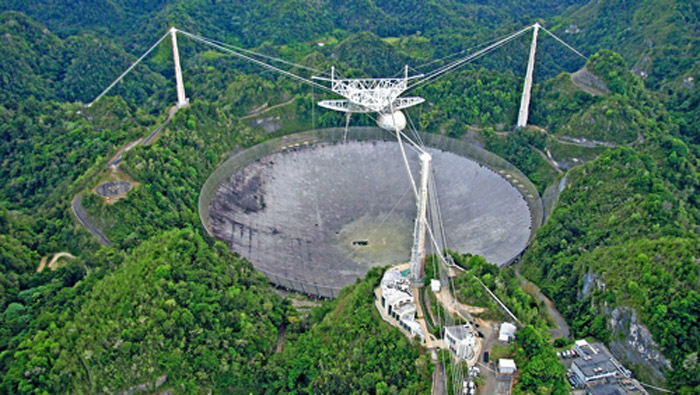
\includegraphics{images/20151101114231-0_8e7cc_c7a44aca_orig.jpg}}
\caption{\label{fig.arecibo} Arecibo telescope, in Puerto Rico.}
\end{subfigure}
\hfill
\begin{subfigure}{.48\textwidth}
\resizebox{\hsize}{!}{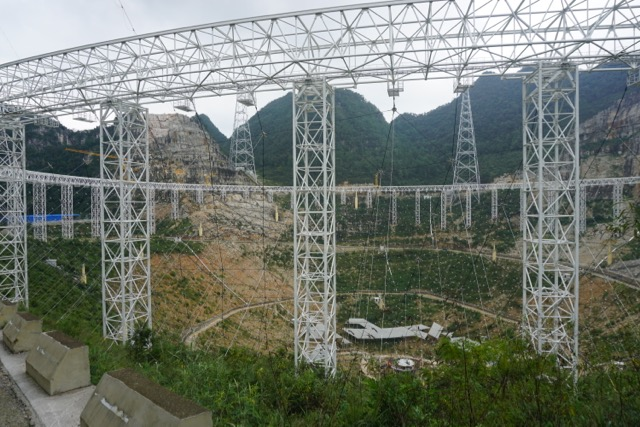
\includegraphics{images/FastTelescope_8sep2015.jpg}}
\caption{\label{fig.FAST} FAST telescope, in China}
\end{subfigure}
\caption{\label{fig.singleDishes} Examples of large single-dish radio telescopes.}
\end{figure}

\section{An Observer's Perspective of Radio Interferometry}

\pg
Astronomers who request observation time on interferometric arrays are generally not experts in the theory and operation of these arrays. This is a simple consequence of scientific division of labour. This thesis is written from the perspective of an ``expert" user: one who specialises in understanding interferometric arrays and reducing their data, rather than their subsequent analysis. However, it can be very helpful to contextualise this perspective in the experience of other scientists, which is what this section aims to do.

\pg
LOFAR data can be acquired through observation or via the Long-Term Archive. The worst of this data will already be flagged. Users can thus generally proceed directly to calibration. Because there is no guarantee of sufficient signal-to-noise in the ``target field" (the object that the astronomer is actually interested in), it is standard practice to observe a calibrator source for 5 minutes before and after each observation. Such sources typically need to be bright and unresolved for the interferometer being used. Because they are bright and at phase centre for the 5-minute observation, the SNR when solving for calibration solutions for these 5 minutes will tend to be quite good. These solutions will then be interpolated between the 5 minutes onto the 8-hour observation. Calibration will be described in \cref{section.calibration}.

\pg
So far, the astronomer will have worked entirely with visibilities. However, generally speaking, the aim will be to get information on the object's brightness distribution at the observing frequency. This will require \emph{imaging}: going from visibilities to the image-plane. This can be done through a variety of tools, but will generally involve deconvolution. Imaging will be the subject of the rest of this chapter, and deconvolution will be described in more detail in \cref{section.clean}.

\pg
After obtaining the initial image, it may be desirable to perform a few rounds of self-calibration \citepads[cf.]{2018arXiv180505266B} on the target field. This consists of extracting a model from the initial image and using it as a new calibration model, then re-imaging. Doing this will usually dramatically improve the final image. 

\pg
The framework for interferometric calibration is complex, and understanding it requires a good grasp on interferometry itself. For now, we will assume that calibration has been performed perfectly, and that the gain-corrections have been applied to the voltage measured by our antennas. We therefore work with the true signal from astrophysical sources until \cref{section.RIME}.



\section{Interferometry: Bypassing the Diffraction Limit}

\pg
There are two quantities of interest to all astronomers: sensitivity and angular resolution\footnote{Other kinds of resolutions - in time and frequency, for example - are also extremely important to many astronomers, but are not what concern us here.}. An instrument's sensitivity is a function of its collecting area\footnote{It is also a function of technological factors, of course, but \emph{ceteris paribus}, a more sensitive telescope means a telescope with a wider collecting area}. Resolution, for well-designed instruments\footnote{By this, we mean that we assume that an instrument is also designed to optimise resolution.}, is limited by diffraction in the absence of atmospheric effects. This introduces specific issues in the radio domain. Radio waves have very long wavelengths - often comparable to meters, rather than the $\sim100-1000$nm wavelengths of optical light. Achieving a resolution comparable to those of optical telescopes would thus require making telescopes with apertures tens of millions of times larger than those already titanic instruments!

\pg
In practice, this technical constraint on resolution is one that astronomers are very interested in overcoming. This technical limitation therefore demands a technical solution. In practice, this solution consists of recourse to interferometric techniques. Indeed, interferometry can be thought of as the construction of a "sparse" dish, as illustrated in \cref{fig.aperture.synthesis}.

\begin{figure}[ht]
\centering
\begin{subfigure}{.43\textwidth}
\resizebox{\hsize}{!}{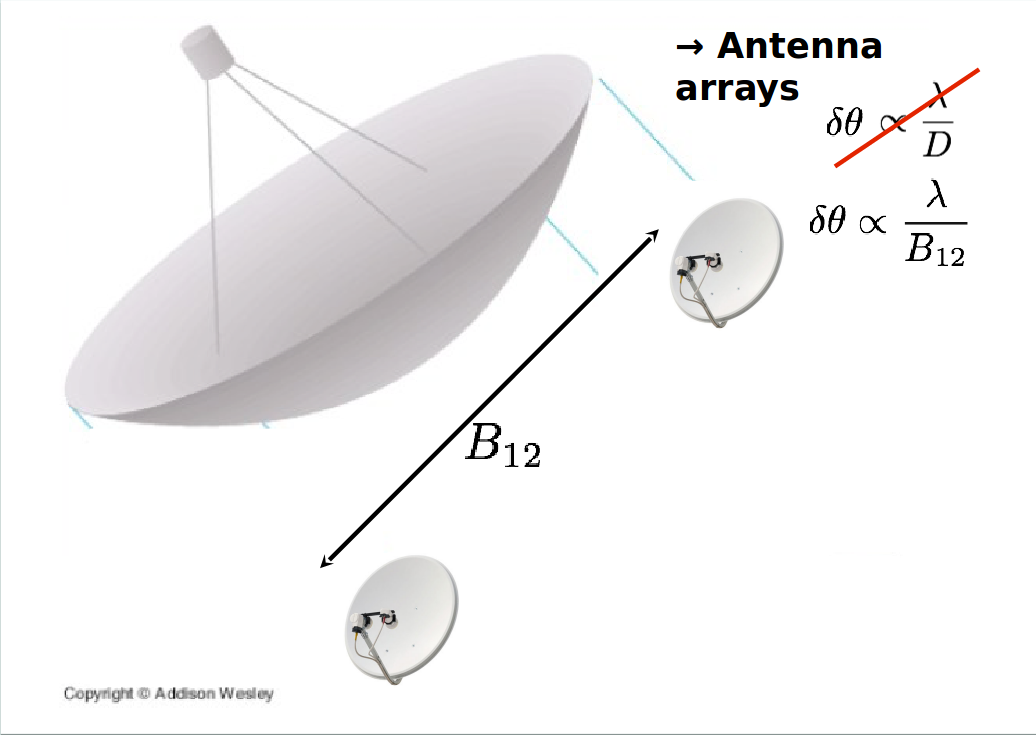
\includegraphics{images/baseline-resolution.png}}
\caption{\label{fig.baseline.image} A pair of dishes can surpass the resolution limit of its components.}
\end{subfigure}
\hfill
\begin{subfigure}{.43\textwidth}
\resizebox{\hsize}{!}{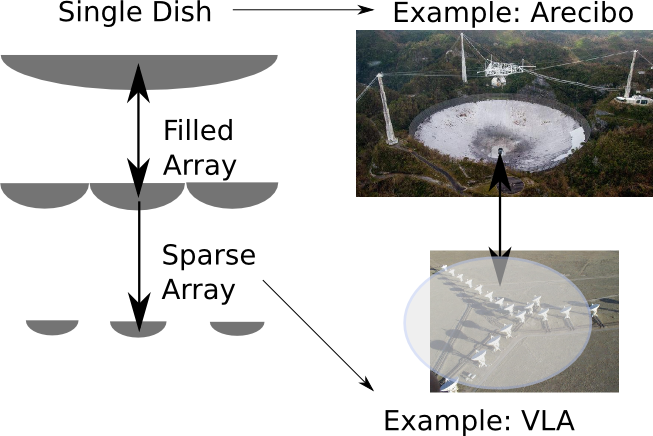
\includegraphics{images/sparseArray.png}}
\caption{\label{fig.arecibo.vla} With enough pairs of dishes, it is possible to synthesise a much larger dish.}
\end{subfigure}
\caption{\label{fig.aperture.synthesis} Illustration of the underlying principle of interferometry. The 27 dishes of the VLA can be thought of as "synthesising" a similar circular dish as Arecibo. This idea is the reason why radio interferometry is historically known as "aperture synthesis" in the literature of radio astronomy. \cref{fig.baseline.image} is copyrighted by Addison Wesley.} % \textcolor{red}{CHANGE FIG B. AS THE ELLIPSE IS NOT SEE-THROUGH}}
\end{figure}

\pg
Interferometric observations follow a very familiar pattern: the elements of the interferometric array (which can be single dishes or phased arrays\footnote{Described in \cref{sec.visibility}} of smaller antennas) measure a voltage. This voltage is correlated between antennas, as will be described shortly. Each of these correlations correspond to a single Fourier mode of the sky, as per the Zernike-van Cittert theorem (cf. \cref{sec.imag.psf}). They must be calibrated, by comparing the observations of a calibrator source and modelled visibilities. Calibration is described in much greater detail in \cref{section.RIME}. Then, the calibrated visibilities are used to reconstruct an image of the sky, which often requires deconvolution due to the sparsity of interferometric arrays.

\pg
The resolution improvement of interferometers does thus not come for free. To better understand the cost of interferometry, we will cover calibration after explaining the particularities of interferometers. We will begin with the properties of their core component: the baseline.

\subsection{The Baseline}

\pg
To define the baseline, we must begin by considering the geometric properties of an interferometric array. For now, let us assume that we are observing the sky above the array, a practice known as drift-scanning. A baseline then consists of the vector subtraction of the positions, in 3-dimensional space, of its two constituent antennas. Note that each antenna pair therefore has 2 corresponding baselines, since for each pair of antennas A and B we create baselines AB and BA. These distance vectors are then divided by the observing wavelength to give a dimensionless set of coordinates, known as $(u,v,w)$. These coordinates define the baseline entirely. 

\subsection{The Visibility}\label{sec.visibility}

\pg
We have defined what a baseline corresponds to: a vector coordinate in $(u,v,w)$-space. To each baseline we associate a measurement, which we call the \emph{visibility}. 
\begin{figure}[ht]
\centering
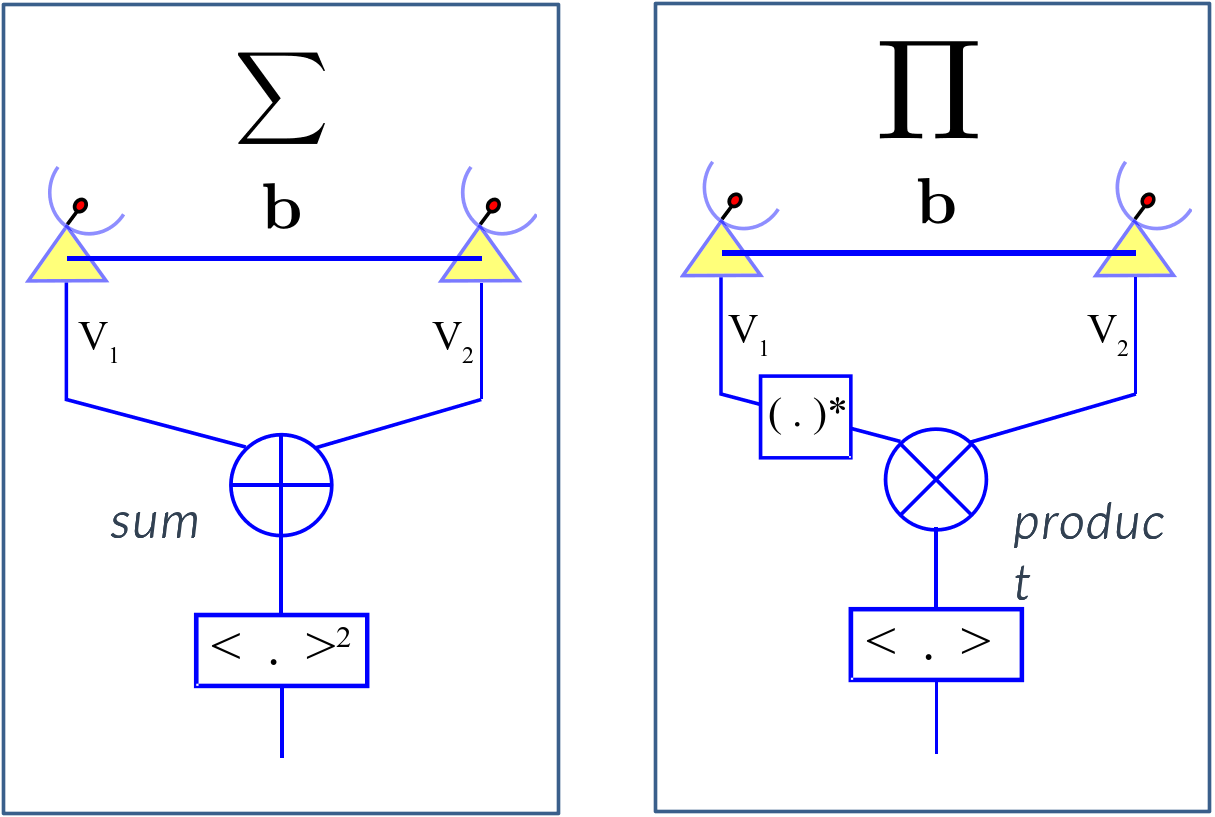
\includegraphics[width=.7\textwidth]{images/visibility-creation.png}
\caption{\label{fig.visibility} There are two ways to combine the voltages from two antennas into a visibility: they are sum-correlation and $\pi$-correlation. In this manuscript, we will only concern ourselves with the latter. Image credit: Julien Girard}
\end{figure}
The visibility associated with baseline $\mathbf{b}_{AB}$ is created by taking the voltage measured by antenna A, multiply it by the complex conjugate of the voltage measured by antenna B, average over the correlator dump time (i.e. the time over which the measurement is made). This scalar quantity is associated to the baseline position vector $\mathbf{b}_{AB}$. In other words:
\begin{align}
\mathbf{b}_{AB} &= \frac{\mathbf{x}_{B}-\mathbf{x}_{A}}{\lambda_\mathrm{obs}}\\
V_{AB}          &= \langle V_{A} V_{B}^*\rangle_{\delta t, \delta \nu} 
\end{align}
where $\langle \cdots \rangle_{i}$ denotes an averaging over quantity $i$. We see that a visibility is a complex vector quantity. We also see that $\mathbf{b}_{AB} = \mathbf{b}_{BA}^*$: the information of the visibility associated with baseline BA is contained in the visibility associated with baseline AB. This means that in practice, only half of the visibilities ever need be stored. What does the visibility measurement correspond to?
\begin{figure}[ht]
\centering
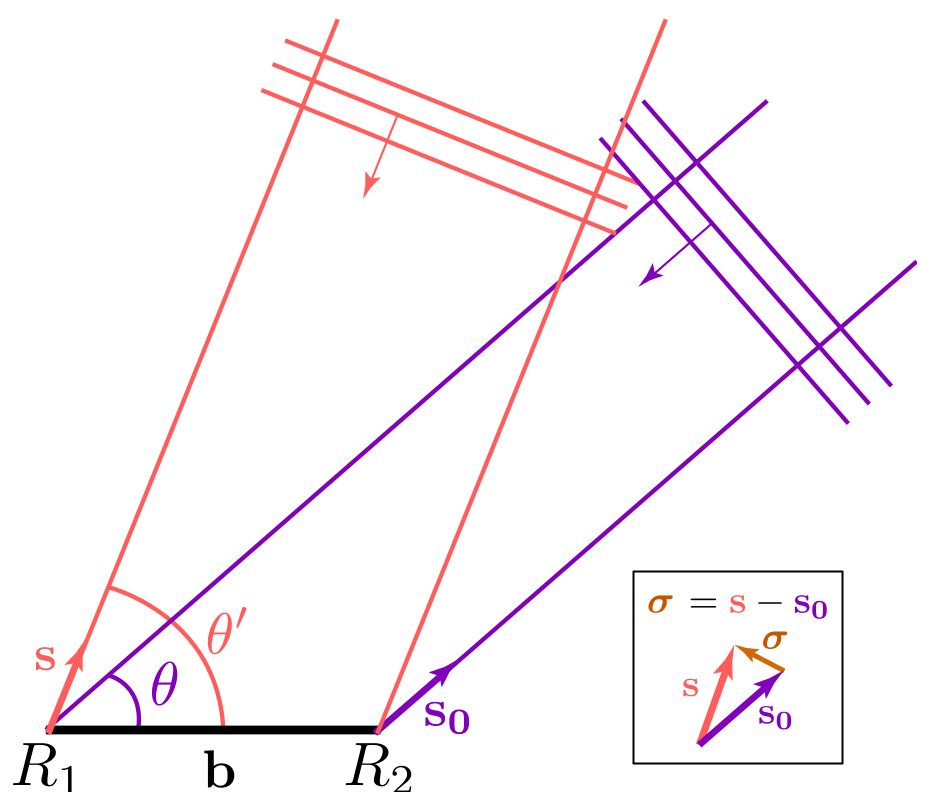
\includegraphics[width=.5\textwidth]{images/visibility-measure.png}
\caption{\label{fig.visibility.measure} Here, we assume that there are only two sources in the sky whose signal can be measured by our antennas. The final visibility is the sum of the visibilities associated with each individual source. Image credit: Julien Girard \textcolor{red}{add reference to julien's phd}}
\end{figure}

\pg
Different astrophysical sources are located very far apart, and so their signals do not interfere. They are measured additively in both antennas. Provided that the signal from both sources is coherent when observed by the dishes, the correlation between the voltages measured by antennas A and B will simply be the sum of the voltage correlations associated with individual sources. This is shown in \cref{fig.visibility}: the radio signal from two different sources, at two different locations, is picked up simultaneously by both radio antennas. Because only the correlation between both antennas is measured, the signals do not interfere. % - i.e. the interferometric signal from different sources are additive.
\pg
Note that in Fig. \ref{fig.visibility.measure}, neither source is at the zenith. This introduces the notion of the \emph{effective baseline} which is shorter than the \emph{physical baseline} when measuring a signal from a source that is not at the zenith. Sources in different positions in the sky will be measured by an interferometric array, but the same array will have different effective baselines for different sources. To point an interferometric array in a specific direction in the sky, one must introduce a phase delay in each antenna (or, for fundamental interferometer elements such as the LOFAR tiles or NenuFAR, by playing with the cable length between each dish and the correlator). This ensures that the constituent antennas' sensitivities are maximised in the direction of interest. The position of sources are then given in terms of the cardinal angle $\sigma$: this is the difference between the position of a source and the phase centre, which is where the array is pointing. For example, in \cref{fig.visibility.measure}, if we point antennas and introduce phase delays such that we are pointing the array towards Source 2, the position of Source 1 will be $\sigma$.

\subsection{The $uv$-plane}

\pg
In general, interferometric design is such that the $w$ component of visibilities' $(u,v,w)$ coordinates is negligible (or can be put in a frame of reference where it can usually be approximated as such). Radio astronomers tend to thus talk of a $uv$-plane rather than $uvw$-space to describe visibility space. The set of $uv$-values for all the baselines of an interferometric array is known as its $uv$-coverage, and defines the array's properties entirely.
For the VLA, for example, the instantaneous $uv$-coverage when observing the zenith will be as shown in Fig. \ref{fig.vla.uvcoverage}.

\begin{figure}[ht]
\centering
\resizebox{\hsize}{!}{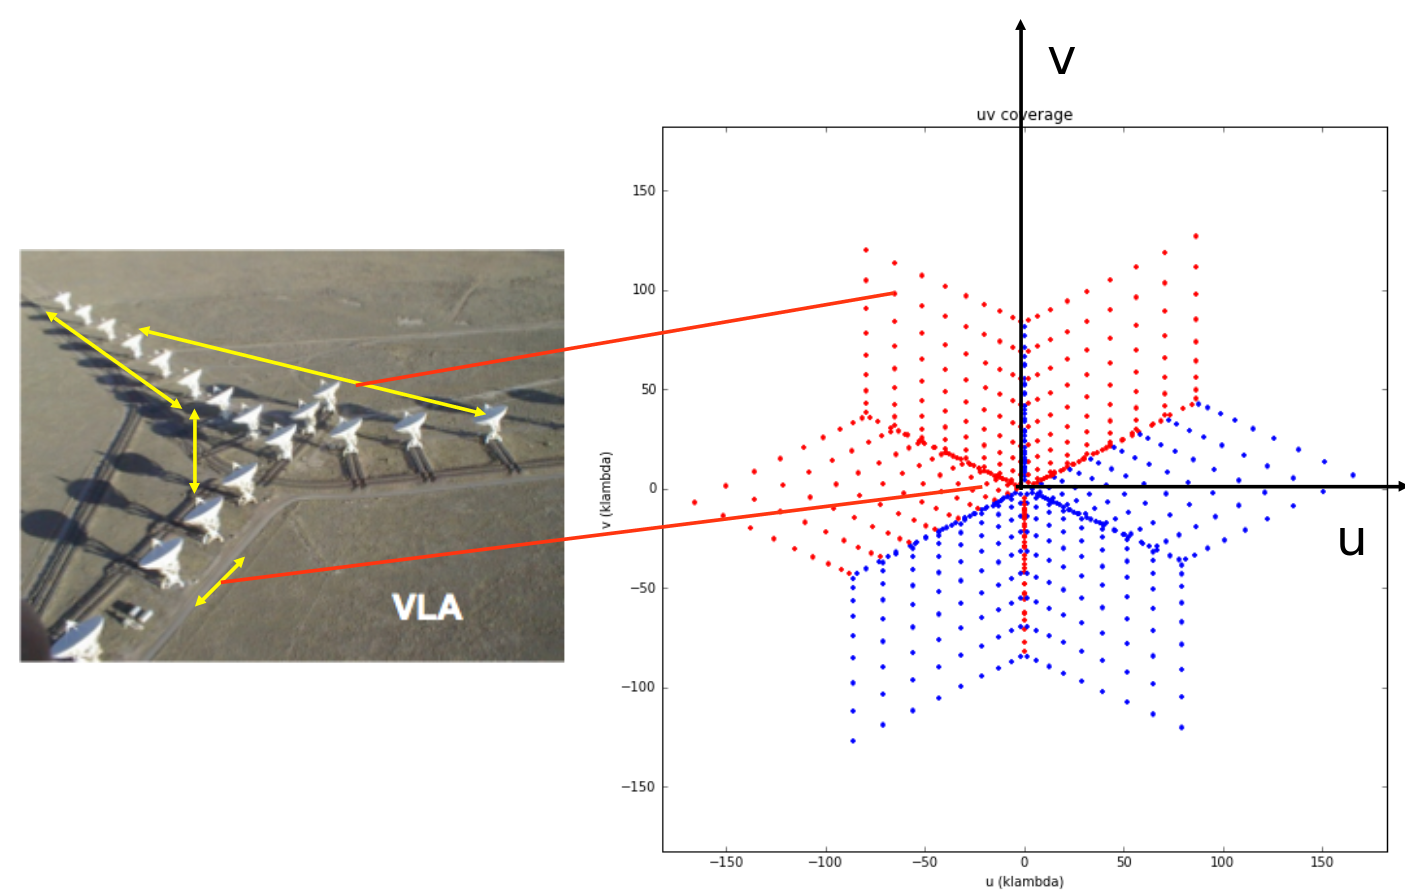
\includegraphics{images/vla-uvcoverage.png}}
\caption{\label{fig.vla.uvcoverage} The VLA contains 27 radio dishes placed as shown above. Each antenna pair between those 27 gives two single baselines, here, one red and one blue. Image credit: Julien Girard}
\end{figure}

%\pg
%The more points an array has in $uv$-space, the greater its $uv$-coverage and the better it will observe. This coverage can be improved for free in two main ways: firstly, the use of a technique known as supersynthesis (since the interferometer "synthesises" a dish at any given time, by assuming that the sky does not evolve over a certain time frame, we can treat different times as measurements of the same sky) and taking advantage of the frequency-dependence of $uv$-coordinates.The impact of both practices will be described in greater detail in \ref{sec.imag.psf}, but know that "$uv$-tracks" simply correspond to the $uv$-coverage of an interferometer observing over some period of time.

\pg
Individual antennas of an array can be pointed mechanically, and so the loss of antenna sensitivity in the direction of interest (and therefore the loss of net interferometric array sensitivity) can be minimised. But what happens to the array itself? It is useful here to go back to the illustration of Fig. \ref{fig.arecibo.vla}. Think of each dish in the array representing a "filled" segment of a massive but empty dish. By projecting our observation in a given direction, this dish goes from circular to elliptical.
\begin{figure}[ht]
\centering
\begin{subfigure}{.40\textwidth}
\resizebox{\hsize}{!}{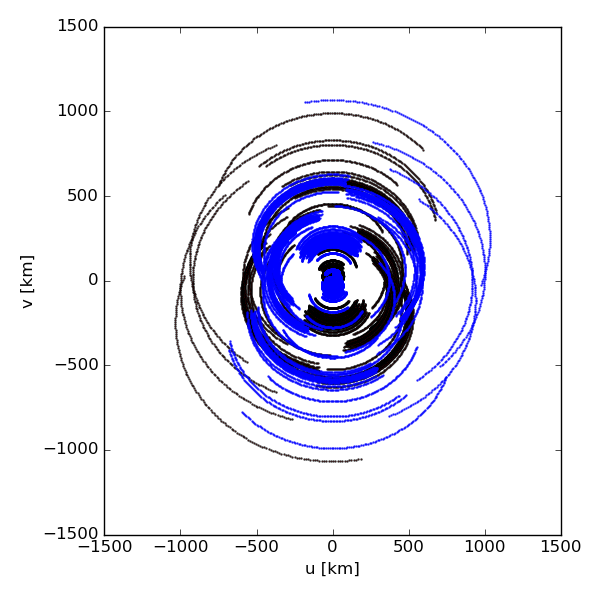
\includegraphics{images/lofar-uvcoverage-zenith.png}}
\caption{\label{fig.lofar.uvcoverage.zenith} $uv$-coverage of an 8-hour LOFAR observation when pointing at zenith.}
\end{subfigure}
\hfill
\begin{subfigure}{.40\textwidth}
\resizebox{\hsize}{!}{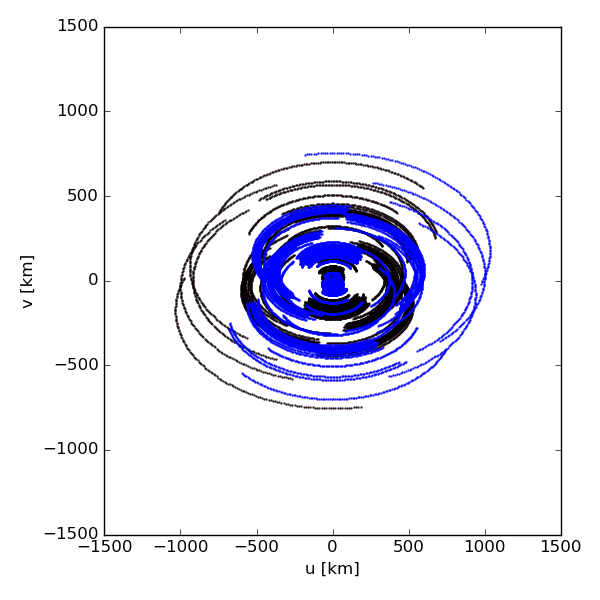
\includegraphics{images/lofar-uvcoverage-elsewhere.png}}
\caption{\label{fig.lofar.uvcoverage.elsewhere} $uv$-coverage of an 8-hour LOFAR observation when pointing 45 degrees away from zenith.}
\end{subfigure}
\caption{\label{fig.uvcoverage.lofar} Effect of array pointing on $uv$-coverage. By pointing the array 45 degrees in the $v$-axis, the array's $uv$-coverage (and thus maximum resolution) is decreased along the $v$-axis. Two colours are used, because $V_{AB}=V_{BA}$, and so only half the visibilities are stored in practice.}
\end{figure}


\subsection{The Point-Spread Function}\label{sec.imag.psf}

\pg
We have seen that the purpose an interferometric array is to overcome the diffraction limit of single-dish antennas. We have described visibilities, which are the quantities measured by an interferometric array. What remains is to describe how these measurements are related to the sky brightness distribution.

\pg
Assuming that all the antennas in an array are equivalent and perfectly calibrated, the van Cittert-Zernike theorem (\citetads{1934Phy.....1..201V}, covered in \citetads{2001isra.book.....T}) allows us to equate a visibility with a single Fourier mode of the plane tangent to the sky where the instrument is pointed. This direction is called the \emph{phase centre}, because phase shifts are introduced between antenna voltages before averaging so as to point each visibility in this direction. 

\pg
The Point-Spread Function (PSF) of an instrument is its point source response: it will determine the angular resolution limit due to the instrument. We know that the Fourier transform of a single point source with unit flux at phase centre is a constant. If we measured the full (infinite) visibility space, then we could reconstitute a point source perfectly. In practice, however, we only ever measure a subset of the visibility space: an interferometric array's PSF is thus the inverse Fourier transform of the array's $uv$-coverage, as these are the only points for which we have information on visibility space. The more elements in the array, the better the $uv$-coverage and thus the better the PSF. An interferometer's PSF will always be worse than an antenna dish of equivalent diameter, the UV-coverage of which is the inverse Fourier transform of a disc. This is because an interferometer behaves like a \emph{sparse} dish: the sparsity of our coverage manifests as very large point-spread function. The more baselines are available, the less sparse the UV-coverage, and so the better the PSF. This is shown in Fig. \ref{fig.vla.PSFvsUVcov}.
\begin{figure}[h!]
\centering
\resizebox{\hsize}{!}{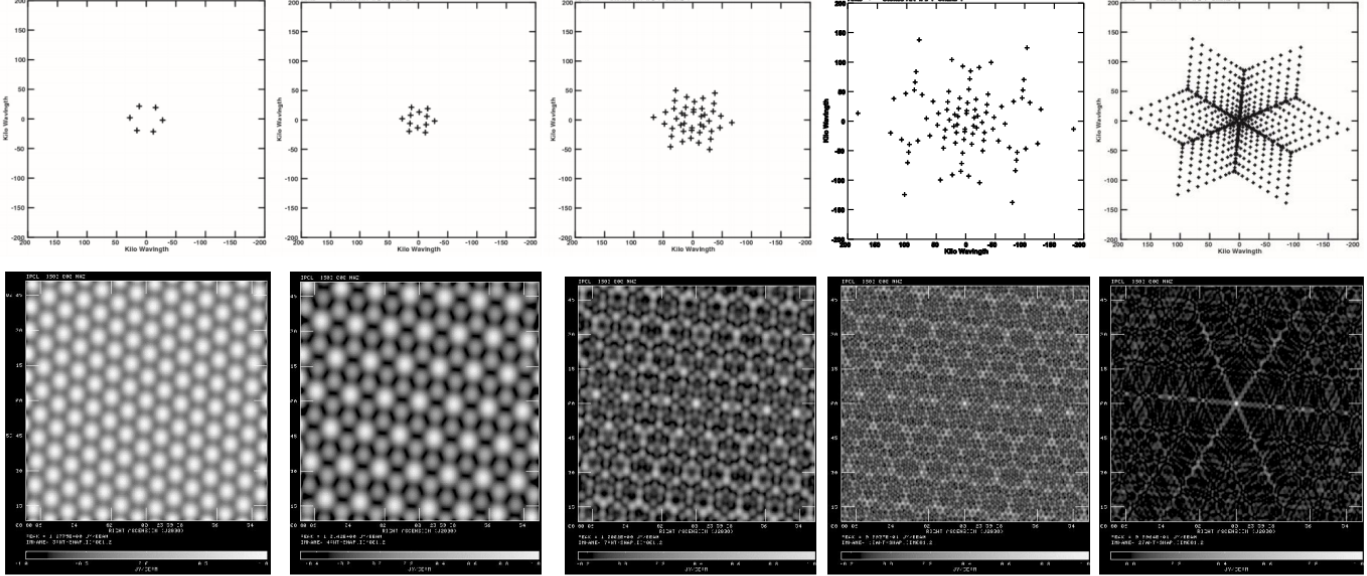
\includegraphics{images/PSFvsUVcov.png}}
\caption{\label{fig.vla.PSFvsUVcov}Plot of the PSF associated to more and more complete UV-coverage (here, consisting of more and more elements of the VLA). Image credit: Rick Perley, 3GC4 lecture.}
\end{figure}

\pg
This PSF can be improved by assuming that the sky is constant over periods of time (supersynthesis) or constant over fractions of the total bandwidth. This improves UV-coverage by a factor $N_\mathrm{t}\times N_\nu$, the number of measurements in time and frequency respectively. The effect of supersynthesis on the PSF is shown in Fig. \ref{fig.vla.PSFsupersynthesis}.
\begin{figure}[h!]
\centering
\resizebox{\hsize}{!}{\includegraphics{images/{PSF_supersynthesis}.png}}
\caption{\label{fig.vla.PSFsupersynthesis}Effect of supersynthesis on the UV-coverage of the full VLA. Image credit: Rick Perley, 3GC4 lecture.}
\end{figure}

\pg
Of course, even with these techniques, the PSF is never perfect, and flux from very bright sources will contaminate the rest of the field. The source in the last image of Fig. \ref{fig.vla.PSFsupersynthesis}, for example, only appears point-like by contrast to the others. If we wish to recover faint emission - and when interested in deep extragalactic fields, that is exactly what we wish to do - then we need to ensure that the effect of the PSF in our images is mitigated, for the brighter sources at least, lest their sidelobes (tails of the PSF convolved with the source) drown out signal from fainter sources. This means \emph{deconvolving} the PSF from radio interferometric images.

\subsection{From Dirty to Clean: Deconvolving the PSF}\label{section.clean}

\pg
Raw images made from radio interferometric data consist of the underlying flux distribution convolved to the array's PSF. The quantity of interest to astronomers is the underlying flux distribution. To recover that information from images, deconvolution is needed.

\pg
In practice, performing a full deconvolution on large images (easily over 25 million pixels in total) is not computationally viable. Scientists therefore resort to algorithms and techniques to accelerate imaging and deconvolution. For example, the use of Direct Fourier Transforms (DFT), which are extremely slow, is avoided when going from visibility space to image space - Fast Fourier Transforms (FFTs) are preferred. Similarly, one seeks to avoid having to perform full deconvolution on the dirty image, since many pixels in the image do not actually contain astrophysical signal. In this chapter, we will briefly cover the most common method of deconvolution used in radio astronomy.

\pg
We use dynamic range (DR) as a quality metric in radio images. DR is the ratio of the flux of the brightest source in the field to the flux of the faintest source in the field.  We define dynamic range as:
\begin{equation}\label{eq.DR.imag}
\mathrm{DR} = \frac{\mathrm{flux}_\mathrm{brightest}}{\mathrm{flux}_\mathrm{faintest}}
\end{equation}
The higher the DR, the deeper we image the sky, and thus the better the image. There are two big constraints to reckon with: firstly, we do not want to deconvolve the PSF from all pixels in the image, but only from those within which large amounts of underlying flux fall. Secondly, if we only deconvolve some pixels rather than performing a full deconvolution, then care must be taken not to treat artefacts in the field (which can be created from overlapping PSF sidelobes from neighbouring sources, even with perfect calibration) as true flux. Doing so would lead to an attempt to deconvolve a PSF from a pixel while assuming an incorrect underlying flux value for this pixel and thus result in the introduction of further artefacts in the image.

\pg
The dominant family of deconvolution algorithms used in radio astronomy at the time of writing is CLEAN\footnote{The other main family of deconvolution algorithms, Maximum Entropy Methods (MEM), are not very widely-used at the time of writing, but remain an active area of research (cf. \citetads{2018ApJ...857...23C}).}. It attempts to optimise for the first requirement while being constrained by the second.The various CLEAN algorithms seek out the brightest pixel(s) in the image, potentially applying a mask to the image first in cases where some \emph{a priori} knowledge on flux distribution is available. It then deconvolves those pixels up to a predefined threshold (either a fraction of the initial pixel value or some factor of the estimated noise value). It does this some predefined number of times. Then, it collects the aggregate \emph{model} (the flux estimate for each deconvolved pixel up to this point), convolves the model with the PSF, and subtracts the result from the dirty image. It then begins to choose the brightest pixels again, and continues to clean until it reaches a stopping condition (usually either a flux value or a maximum number of iterations).

\begin{figure}[h!]
\centering
\resizebox{\hsize}{!}{\includegraphics{images/{dirty-vs-clean}.png}}
\caption{\label{fig.vla.clean} Effect of MetroCLEAN algorithm on a dirty image of 3C295. To the left, the dirty image; to the right, the deconvolved image (same size, resolution \& flux scale, made with the same data). As we can see, the latter is much more scientifically interesting.}
\end{figure}


\pg
In Fig. \ref{fig.vla.clean}, we show the effect of deconvolution on a dirty image of 3C295 (a very bright \& complex source which is the subject of much of this thesis' work). Since this source includes diffuse emission, standard CLEAN is insufficient (since CLEAN assumes a sparse distribution of point-like sources). Instead, the DDFacet software package's novel MetroCLEAN algorithm (see \citetads{2017arXiv171202078T}), which deconvolves islands consisting of sets of pixels at once, was used. This allowed for a far greater dynamic range than standard CLEAN could achieve.

\pg
The problem of imaging radio interferometric data is still a very active field of research today. For more information on this topic, the NRAO website\footnote{See \href{https://www.cv.nrao.edu/~abridle/deconvol/node8.html\#SECTION00051000000000000000}{the CLEAN section of the NRAO website}.} is an excellent start for a general introduction to this topic, while \citet{2017arXiv171202078T} provides an outstanding entry point for cutting-edge work at the time of writing.


\section{Weighting Schemes}
\pg
In \cref{section.clean}, we discussed the problem of deconvolution in radio interferometric imaging. One consideration that is not raised is the issue of conditioning. Consider two extreme cases: a field containing a few point sources(\cref{fig.point}), and a field containing a diffuse and turbulent source, with very complex flux distribution at all scales (\cref{fig.cyga}). Deconvolving the PSF from the first image using CLEAN algorithms will be child's play, but doing the same with the second will be extremely complex. The first case is said to be well-conditioned, and the second to be poorly-conditioned.

\begin{figure}[h!]
\centering
\begin{subfigure}{.45\textwidth}\resizebox{\hsize}{!}{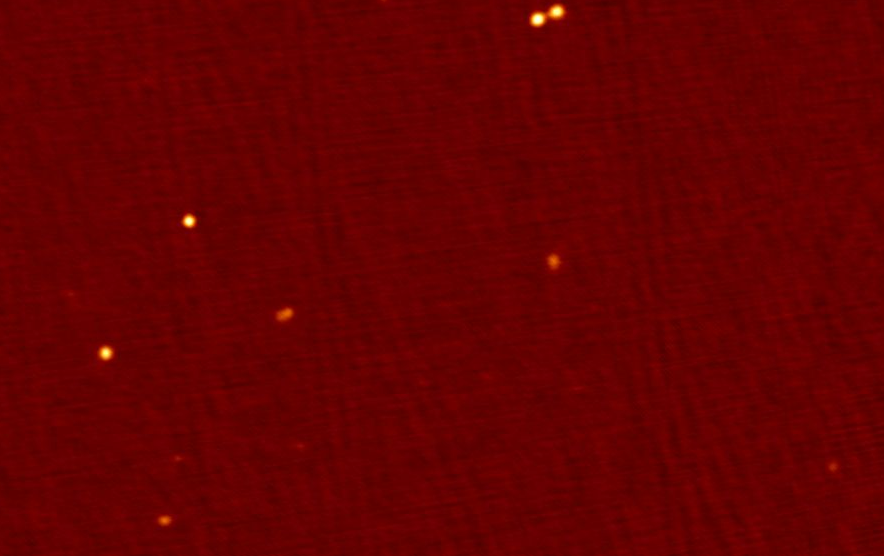
\includegraphics{images/egs-prelim.png}}
\caption{\label{fig.point} Part of the LOFAR field near the Extended Groth Strip as seen by LOFAR.}
\end{subfigure}
\hfill
\begin{subfigure}{.53\textwidth}
\resizebox{\hsize}{!}{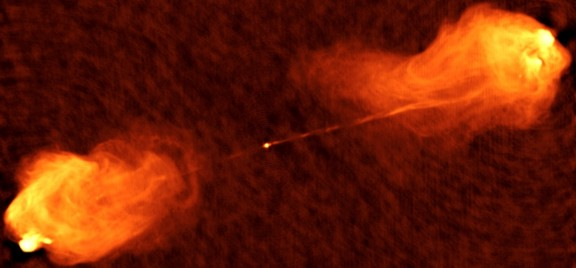
\includegraphics{images/cyga.jpg}}
\caption{\label{fig.cyga} Cygnus A as seen by the VLA. \href{http://images.nrao.edu/110}{Image courtesy of NRAO/AUI}}
\end{subfigure}
\caption{\label{fig.conditioning} Two extreme examples of good and poor conditioning. \cref{fig.point} shows a field with a few point-like sources. \cref{fig.cyga} shows a very complex \& diffuse structure.}
\end{figure}

\pg
The better the conditioning, the easier the deconvolution and the closer to the ground truth its result. As such, when the true underlying structure of a source is poorly-known, getting the best conditioning possible for deconvolution becomes a key concern. Thankfully, because the actual measurements taken with interferometers are the Fourier modes of the sky brightness distribution, they can be weighted when reconstructing the images to fulfill specific requirements. In particular, Briggs weighting \citepads{1995AAS...18711202B} gives a sliding parameter between \emph{natural} weighting, where each visibility is weighed equivalently (this optimises noise in the field) and \emph{uniform} weighting, which gives each visibility a weight inversely proportional to $uv$-plane density. Uniform weighting optimises for resolution at the cost of image signal-to-noise.

\begin{figure}[h!]
\centering
\begin{subfigure}{.48\textwidth}\resizebox{\hsize}{!}{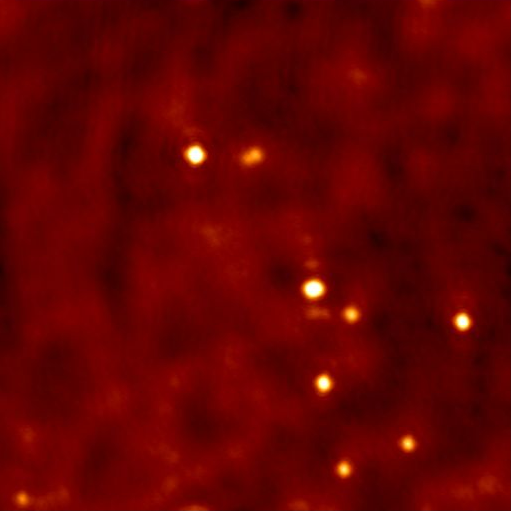
\includegraphics{images/natural.png}}
\caption{\label{fig.natural} Image made with LOFAR data and natural weighting.}
\end{subfigure}
\hfill
\begin{subfigure}{.48\textwidth}
\resizebox{\hsize}{!}{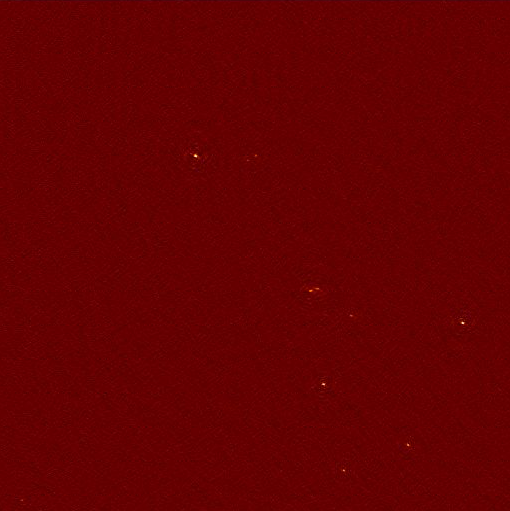
\includegraphics{images/uniform.png}}
\caption{\label{fig.uniform} Image made with the same data as \cref{fig.natural} and uniform weighting.}
\end{subfigure}
\hfill
\begin{subfigure}{.48\textwidth}
\resizebox{\hsize}{!}{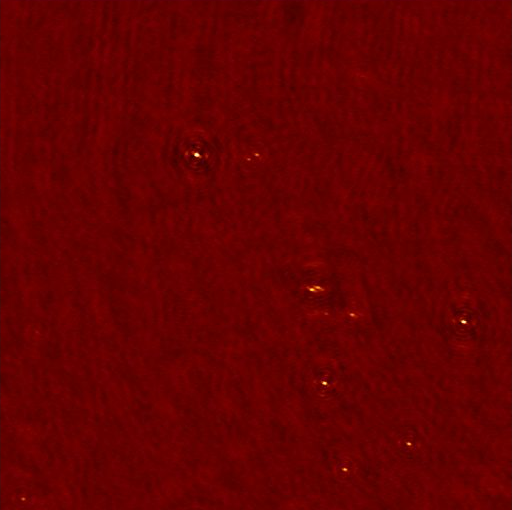
\includegraphics{images/briggs0.png}}
\caption{\label{fig.briggs0} Image made with the same data as \cref{fig.natural} and Briggs weighting, with a Briggs parameter of 0.}
\end{subfigure}
\caption{\label{fig.briggs-weighting}Impact of different weighting schemes on interferometric image reconstruction. All the images shown above are deconvolved.}
\end{figure}

\pg
\cref{fig.briggs-weighting} clearly shows that imaging done with the same data but different weighting schemes give radically different deconvolved images. Images made with uniform (\cref{fig.uniform}) or Briggs (\cref{fig.briggs0}) weighing are much sharper, with uniform weighting (\cref{fig.uniform}) giving such resolution that the sources are nearly invisible in the field (though they are present - the contrast was not upped so as to show all three images on the same flux scale). 

\pg
%Note that the weighting schemes shown here rely only on a choice between normalising visibilities by local $uv$-density vs. signal-to-noise, with Briggs weighting providing a formal method for going from one regime to another or optimising between both. Other weighting schemes exist - one can attempt to optimise data size vs decorrelation\footnote{As data is averaged, decorrelation becomes more and more important in the field. See \cref{section.RIME} for more details.}, for example \citepads[see]{2016MNRAS.462.2542A}. This can help ensure a homogeneous conditioning of the deconvolution problem in the image, by ensuring that the PSF is as peaked as possible throughout the field of interest. Part of the work of this thesis was in devising a weighting scheme dependent on calibration quality, to drastically improve deconvolution conditioning and final image quality. This weighting scheme is described in much greater detail in \cref{chapter.paper}.

\pg
We close this section by noting that data flagging can be considered a form of weighting scheme. This consists of assigning a null weight to those data points considered too corrupted by various instrumental or atmospheric effects (typically, Radio Frequency Interference - RFI - cf. \citetads[cf.]{2010ascl.soft10017O} for an example) to be scientifically useful. Those weights which are not deemed too corrupted are assigned a unit weight. This corresponds to simply dropping those data points which would corrupt the image reconstruction by introducing unphysically strong fringes in the image.

\pg
Flagging is also useful to remove corrected visibilities for which near-zero gains are found: the associated corrected visibilities will consist of some number divided by a near-zero number, for which numerical errors can introduce very large errors. ``Clipping" these visibilities after calibration helps improve the final images.
\clearpage
% !TeX spellcheck = en_UK

\section{Calibration Methods in Radio Interferometry}\label{section.calibration}
\pg
In this section, we will discuss the implementation of interferometric array calibration. Our analysis is based on the RIME formalism, described in \cref{section.RIME}. One key metric of calibration quality is the \emph{dynamic range}, mentioned in Sec. \ref{section.clean}. High dynamic ranges mean that a high contrast has been obtained, and fainter sources can be reached. Here, we redefine dynamic range as follows
\begin{equation}\label{eq.DR}
DR = \frac{flux_{max}}{\max(\sigma_{thermal},\sigma_{artefacts})}
\end{equation}
where $flux_{max}$ is the flux of the brightest source, $\sigma_{thermal}$ the thermal noise in the image, and $\sigma_{artefacts}$ the noise associated with calibration artefacts. This gives a definition for dynamic range useful even in fields with a single source. We can thus use it as a metric for calibration quality specifically.

\pg
The distinction between these two noise sources is crucial; one can never go `below noise' for a given observation, no matter the quality of calibration. Astronomers typically observe for longer periods of time in order to reduce $\sigma_{thermal}$ in their images, but this will not reduce the artefacts caused by poor calibration solutions. Uncorrected Direction-Dependent Effects will not go away on their own, no matter how long the integration time. Similarly, there is a limit to how much improving calibration will improve the final image: eventually, more data is required to drive noise down.

\pg
There are three `generations' of calibration methods, of increasing complexity. We will describe them in terms of the RIME, showing how each generation increases in generality to account for more exotic effects. They are referred to interchangeably as `nth-generation calibration' or `nGC' methods.

\subsection{Generational Analysis}

\subsubsection{First-Generation: Open-Loop Calibration}\label{section.calibration.1gc}

\pg
First-generation calibration methods (1GC methods) consist of open-loop calibration. This relies entirely on instrument stability, and thus imposes significant design constraints on radio telescopes. It consists of briefly observing a calibrator before and after each observation run to find a gain factor and offset error\footnote{For a concrete example, see \href{http://www.analog.com/en/analog-dialogue/articles/open-loop-calibration-techniques.html}{the open-loop calibration techniques page of analog.com}.}

\pg
Phase calibration in the 1GC era `proper' was not necessary, as engineers were capable of ensuring adequate phase stability in contemporary interferometers. Phase was thus calculated relative to a fixed frame of reference, usually the central antenna of a 3-antenna array. 

\pg
In RIME terms, this consists of solving for a very basic form of $\Gjones_p$:
\begin{equation}
\Gjones_p = \begin{bmatrix} a_p t + b_p \end{bmatrix} % \begin{bmatrix} e^{2 \pi i \nu ( \phi_p - \phi_0)} \end{bmatrix}
\end{equation}
where $a_p,b_p$ are constants solved for during open-loop calibration and $t$ is time. %, $\nu$ the observing frequency, $\phi$ the phase at an antenna, and $\phi_0$ the phase at the reference antenna.

\pg
While values for $a_p$ and $b_p$ can in theory be found for both autocorrelation and both crosscorrelations, low signal-to-noise means that in practice, a single set of values is solved for per antenna\footnote{This reduces calibration to solving only for the intensity gains: the data can then only be used for \emph{intensity mapping} (e.g. \citepads{1957IAUS....4..159J}). This practice therefore precludes polarimetry.}. With these techniques, one can achieve dynamic ranges of about 100:1 (\citepads{2010A&A...524A..61N}).

\subsubsection{Second-Generation: Self-Calibration}\label{section.calibration.2gc}

\pg
Second-generation calibration methods (2GC methods) are defined by \emph{self-calibration}\footnote{On the discovery of self-calibration and its evolution in parallel to adaptive optics, see the chapter titled "The Almost Serendipitous Discovery of Self-Calibration'' in "\href{http://library.nrao.edu/public/collection/02000000000280.pdf}{\citep{serendipitous}}.}, commonly referred to as \emph{self-cal} (\citepads{1984ARA&A..22...97P}). As described in \cref{section.RIME.FullSky.CVZ}, this method can only be deployed if the brightness matrix of the sky is the same for all baselines\footnote{This is not to say that the brightness matrix must contain only point sources, but rather that moving our interferometer 500m to the East should not change its measured visibilities} (i.e. that we are not affected by direction-dependent effects).

\pg
The first instance of self-calibration (and adaptive optics in radio interferometry) is a paper published in the era of 1GC by Jennison \citepads{1958MNRAS.118..276J}, expanding on his PhD work, which was published in 1951). With sufficient signal-to-noise, he showed that \emph{phase closure} could be calculated and errors due to the atmosphere thus mitigated.

\pg
Self-calibration and adaptive optics are the same thing, albeit meeting different constraints. Most notably, interferometric data is digital, allowing radio astronomers to perform their adaptive optics correction after the observation.

\pg
If amplitude and phase gains can be written as antenna-dependent, then each antenna-based error is estimated N times (once per baseline which includes this antenna). By estimating, and correcting for, these errors, one can use a simple source model to infer an improved one. This is why the method is referred to as self-cal; by calibrating `on' a good calibrator source (bright, compact and unresolved), one can drastically improve one's source model, along with one's calibration solutions.


\begin{figure}[h!]
\centering
\resizebox{\hsize}{!}{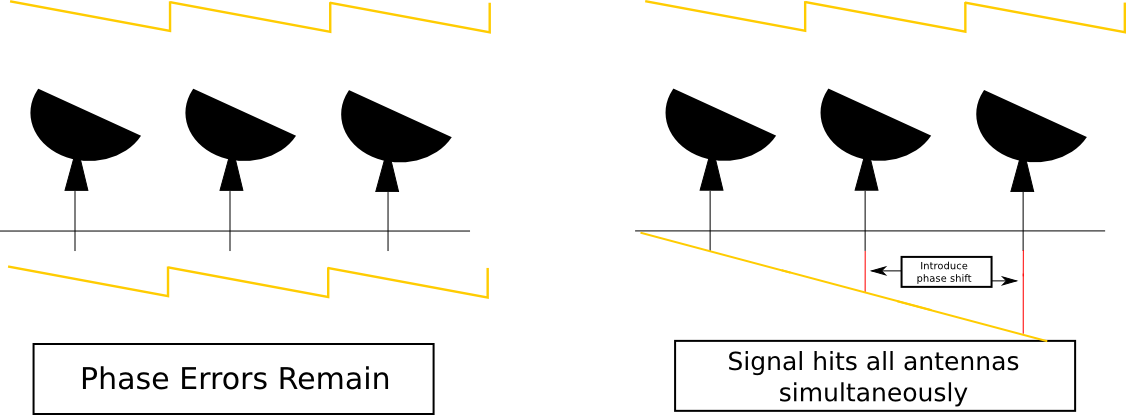
\includegraphics{images/selfcal.png}}
\caption{\label{fig.selfcal} Representation of self-calibration as adaptive optics}
\end{figure}

\pg
By extending this idea to VLBI\footnote{e.g.  \citepads{1974ApJ...193..293R}}, \emph{amplitude closure} was introduced to the field along with phase closure \citepads[as described in][]{1983Sci...219...51R}. These quantities are immune to antenna-based effects.%Astronomers were quick to apply these methods to interferometers in general.

\pg
The great advantage of radio interferometry over optics, however, is that we can \emph{iterate} over progressively improved source models. This is because interferometric data is digital, and because we record phase information.

\pg
In practice, of course, self-cal will be limited by noise. More precisely, it will be limited by sensitivity, in the form of the signal-to-noise ratio (henceforth SNR). For sufficiently bright sources, with high SNR, self-calibration can easily improve dynamic range by a factor of 10 (\cite{serendipitous}, p. 154) in a single iteration. 

\subsubsection{Third-Generation: Direction-Dependent Effects}

\pg
Third-generation calibration (3GC) is an extension of 2GC calibration which takes direction-dependent effects into account. At the time of writing, this is the cutting edge in radio interferometric calibration.

\pg
In this section, I will discuss the approach taken by \textcolor{red}{[cite DDF and kMS paper when it comes out]} and \textcolor{red}{[cite prefactor paper if/when it is out]}, \emph{facet-based calibration}. This method has an imaging equivalent \citepads[see][and associated papers]{2017arXiv171202078T}. The approach cannot be divorced from imaging, for the simple reason that solving for and applying Jones matrices in different directions requires image-plane knowledge of the sky brightness distribution $\Bmatrix$. % The imaging challenges this methods introduces will be discussed in [href to relevant imaging section].

\begin{figure}[ht]
\centering
\resizebox{\hsize}{!}{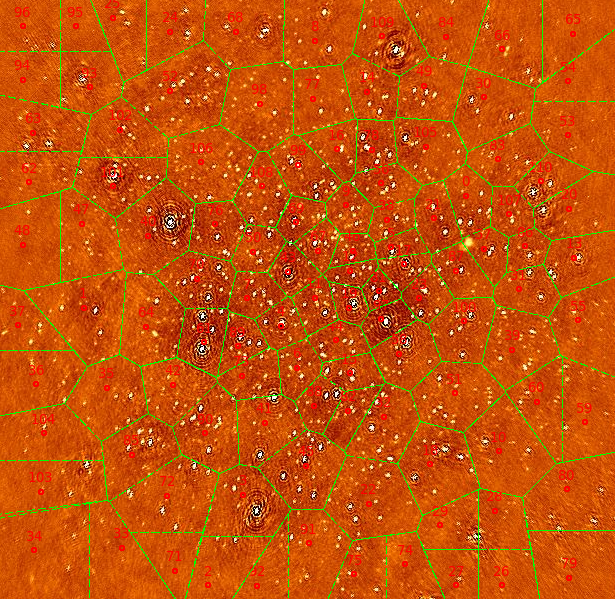
\includegraphics{images/bootes-image.png}}
\caption{\label{fig.facets} Voronoi facets, as implemented in DDFacet. Image is made before application of direction-dependent correction. This is an image of the Bootes field, made by Cyril Tasse.}
\end{figure}

\pg
When performing first and second-generation calibration, one solves for a set of Jones matrices or parameters thereof. Direction-independent calibration then consists of applying these calibration solutions to the visibilities directly. However, while these solutions will be correct in the direction of the calibrator source, they are increasingly likely to be wrong as a function of distance from said calibrator source. The difference between the true gains in a given direction and the gains estimated from the calibrator source are called \emph{differential gains}.

\pg
Why then not solve for a set of calibration solutions for each source in the calibration model, iteratively adding new sources to this model as they become above the noise as calibration artefacts - introduced by poor calibration - decrease? There are two main reasons for this: firstly, the signal-to-noise when calibrating using very faint source models will be poor. This means that gains will likely be extremely noisy, and applying them will result in increased calibration artefacts in the final image. Secondly, even by optimising for signal-to-noise and only using a few of the brightest sources in the field, the problem quickly becomes intractably large in terms of computing power required, provided that standard complex differentiation is used \citepads[see][]{2016ApJS..223....2V}. Wirtinger differentiation \citepads[see][and associated papers]{2014arXiv1410.8706T} does alleviate this somewhat, but is not implemented in all standard direction-dependent calibration software at the time of writing.

\pg
The crucial insight of a faceting approach is then to split the image into a set of \emph{facets}, solving for a set of calibration solutions for each of these facets. These solutions are then applied to the visibilities when mapping them onto the dirty image. The faceting in DDF is shown in \cref{fig.facets}. The facet distribution shown in \cref{fig.facets} encourages an even flux distribution in multiple facets, and ensures that no facet is so small that too little signal would be available within. As we can see from \cref{fig.DDcal.effect}, direction-dependent calibration can drastically improve the quality of wide-field images. It currently represents the state of the art in interferometric calibration. 

\begin{figure}[h!]
\centering
\begin{subfigure}{\textwidth}
\resizebox{\hsize}{!}{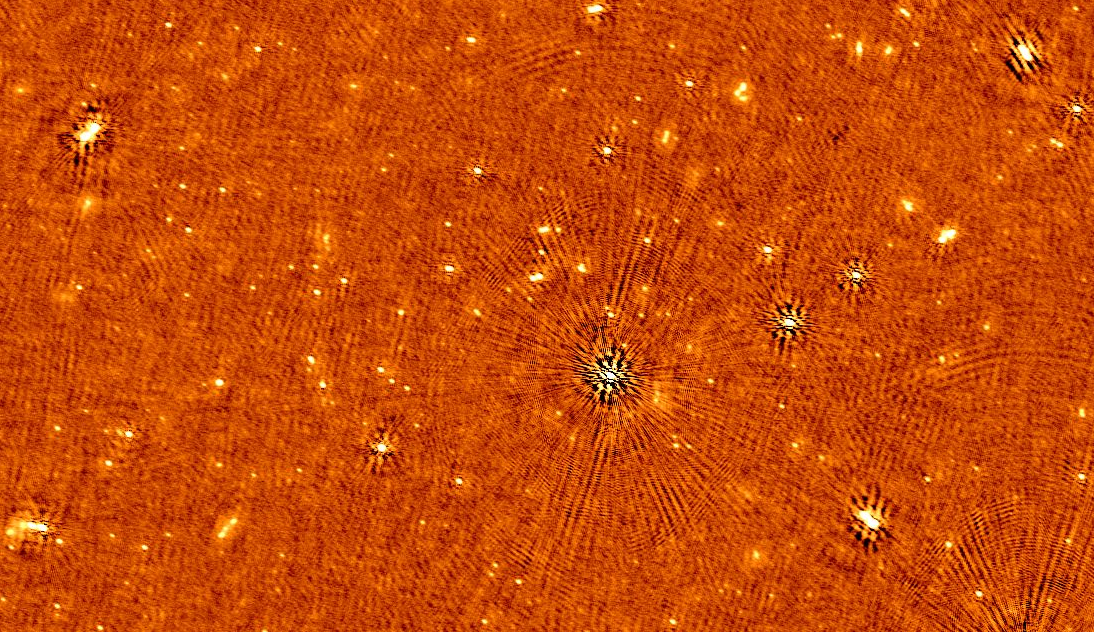
\includegraphics{images/lofar-nocorr.png}}
\caption{\label{fig.lofar.noDDcal} Image of the Boötes field, made without direction-dependent calibration. Image by Cyril Tasse.}
\end{subfigure}
\begin{subfigure}{\textwidth}
\resizebox{\hsize}{!}{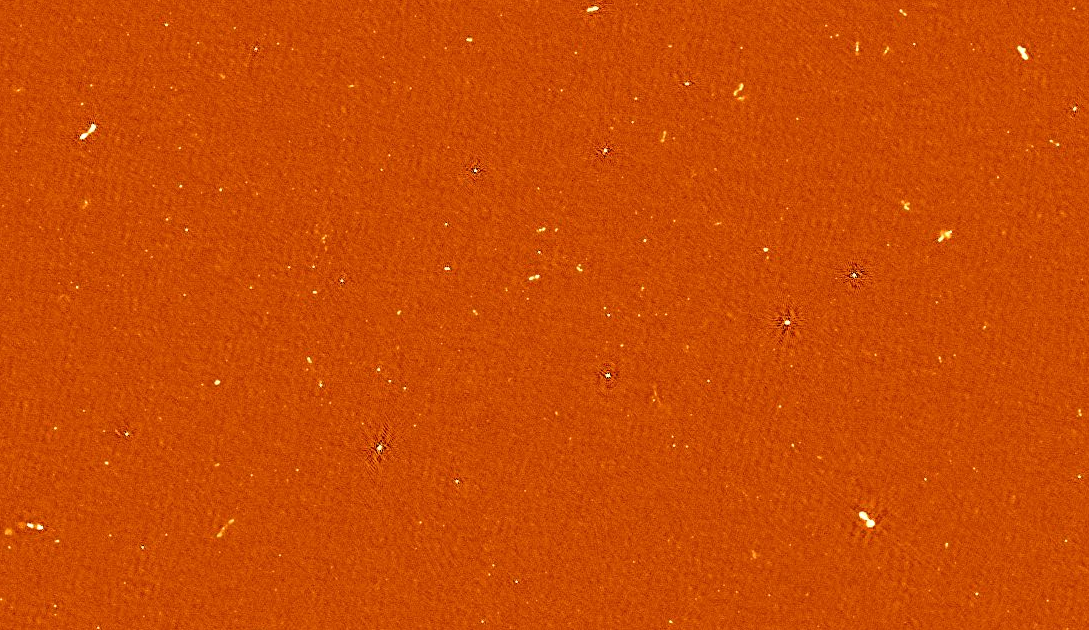
\includegraphics{images/lofar-corr.png}}
\caption{\label{fig.lofar.withDDcal} Image of the same Boötes field, made with direction-dependent calibration. Image by Cyril Tasse.}
\end{subfigure}
%\hfill
\caption{\label{fig.DDcal.effect} Difference between imaging made with (Fig. \ref{fig.lofar.withDDcal})and without (Fig. \ref{fig.lofar.noDDcal}) third-generation calibration.}
\end{figure}








\clearpage

\section{The Low-$\nu$ Sky: Emission Mechanisms}
\pg
This section aims to bring a brief introduction to the emission mechanisms which dominate at low frequencies, and thus determine the physics accessible to extragalactic astronomers working in this band. Specifically, it will briefly describe thermal radiation detected at low frequencies (associated with dust \& protoplanetary disks, and therefore a tracer of star formation) along with free-free radiation (which is emitted from ionised plasma outflows, and thus a tracer of various physical objects e.g. young stellar objects - cf. \citet{2017ApJ...834..206C} - and starburst regions - cf. \citet{2015A&A...574A.114V}) and synchrotron radiation, which is a tracer of more violent and energetic processes (and thus associated with supernova remnants, AGN, or radio halos - cf. \citet{2010A&A...509A..68C}).

\pg
Of course, each individual galaxy will have differing contributions from different mechanisms - in practice, when studying galactic populations, the overall flux at a given frequency will simply be summed up for each galaxy and become one point in a Spectral Energy Distribution, or SED. However, when studying individual objects, it can be critical to understand which emission mechanism dominates at what frequencies. %: it will be very difficult to find traces of star formation in the emission from a galaxy dominated by an AGN, for example. Along with a brief introduction of the main emission mechanisms, then, we will give the characteristic spectrum of each, to show how different types of emission can be differentiated in practice.
For example, the radio and far-infrared spectrum for nearby M82 are shown in Fig. \ref{plot.m82.spectrum}\footnote{Figure and work taken from the NRAO website. For further information, \href{https://www.cv.nrao.edu/course/astr534/FreeFreeEmission.html}{see here}}.
\begin{figure*}[!h]
\centering
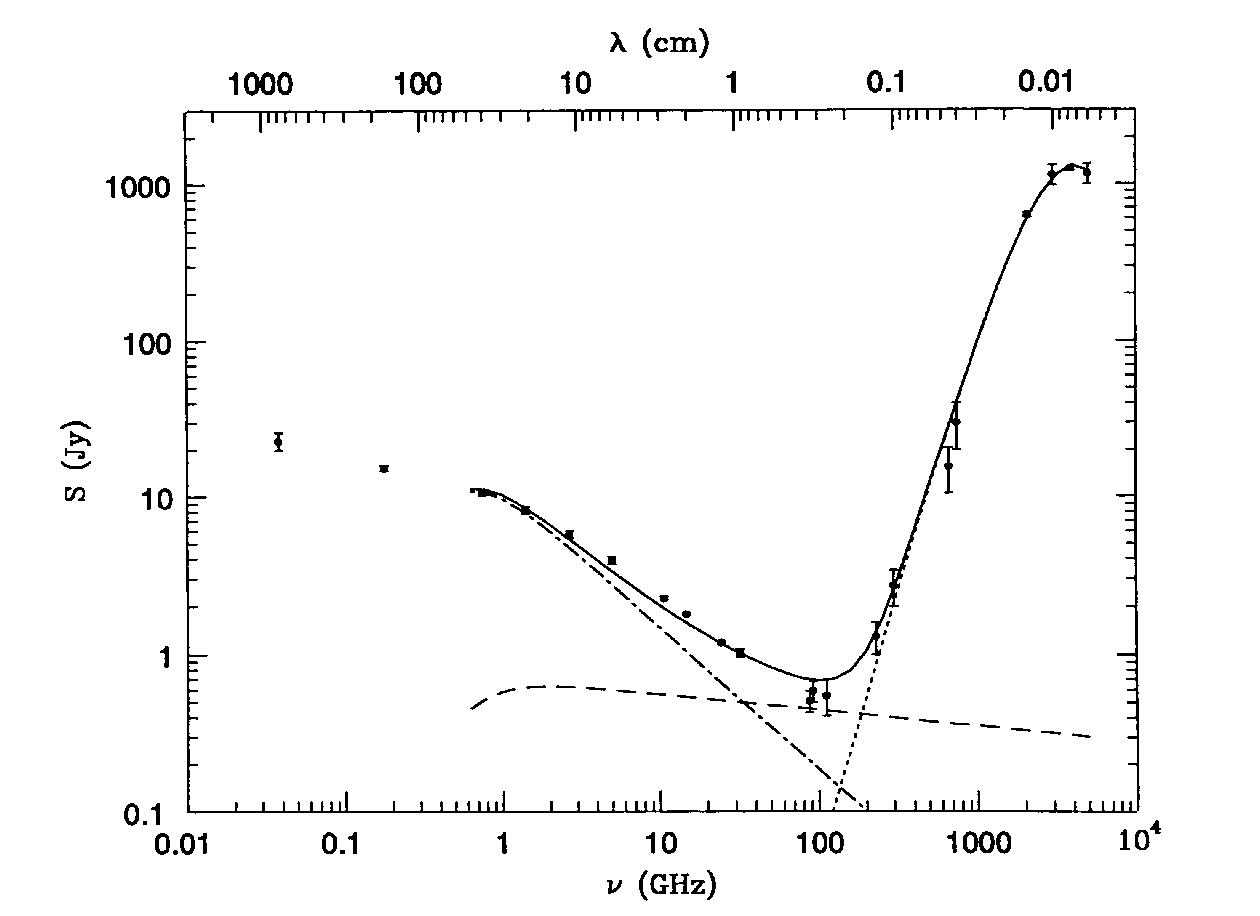
\includegraphics[width=\textwidth]{images/M82Spectrum.png}
\caption{\label{plot.m82.spectrum} Radio and far-infrared spectrum for galaxy M82, as estimated \href{https://www.cv.nrao.edu/course/astr534/FreeFreeEmission.html}{by the NRAO online course}. The flat curve corresponds to free-free emission, while synchrotron radiation and thermal dust emission dominate at low and high frequencies respectively.}
\end{figure*}

\pg


\subsection{Thermal Radiation}
\pg
Also known as black-body radiation, its spectral intensity is given by Planck's law, given in Eq. \ref{eq.planck}.
\begin{equation}\label{eq.planck}
%B_\lambda (\lambda,T) = \frac{2hc^2}{\lambda^5}\left(e^{\frac{hc}{\lambda k_BT}}-1\right)^{-1}
B_\nu(\nu,T) = \frac{2h\nu^3}{c^2}\left(e^\frac{h\nu}{k_BT}-1\right)^{-1}
\end{equation}
where $B_\lambda$ is the flux density at frequency $\nu$ for a source with temperature $T$, and $k_B=1.381 \left[J/K\right]$ is the Boltzmann constant. Near protostellar disks, synchrotron emission is absorbed by the ambient interstellar medium, heating it up to an average of $\sim 10^4$ (see \citetads{2009ApJS..181..255A}, \citetads{1978ppim.book.....S} and references therein). This gives the following spectral curve:

\begin{figure*}[!h]
\centering
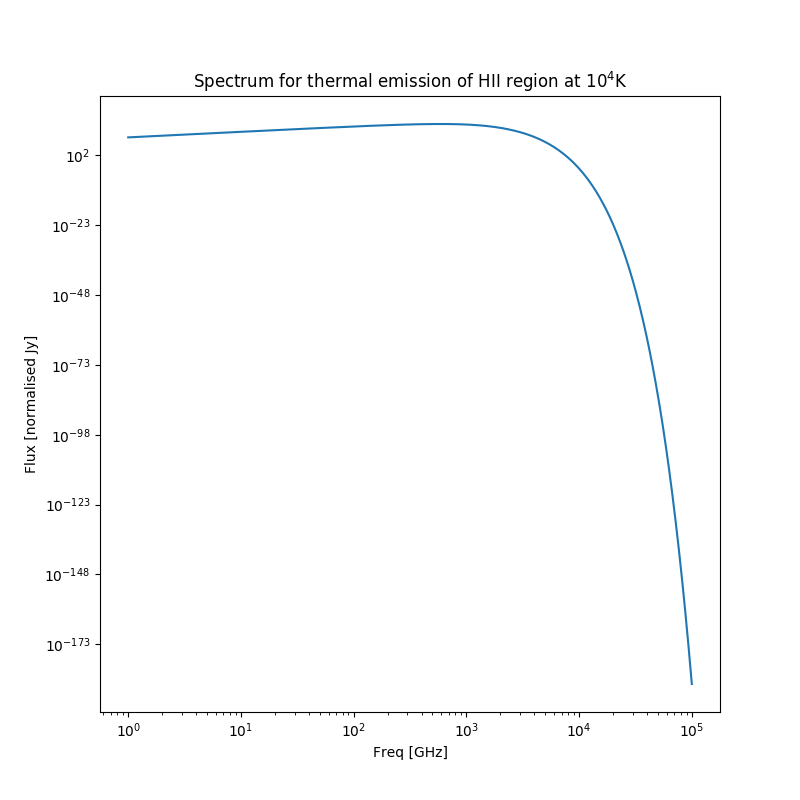
\includegraphics[width=0.8\textwidth]{images/ThermalEmission.png}
\caption{\label{plot.thermal}Log-Log plot of blackbody radiation emitted by a particle at $10^4$ Kelvin. Note that the y-axis is arbitrary, since it will in practice be modulated by the number of particles in a region, radiation efficiency, resolution etc.}
\end{figure*}
\pg
This is the dominant mode of emission for distant galaxies in the infrared band. In the LOFAR regime, it is not expected to dominate for extragalactic sources, but ought to be detected for resolved galaxies.

\subsection{Free-Free Radiation}
\pg
Free-free or ``bremsstrahlung" (``braking") radiation occurs when the trajectory of a high-energy charged particle is deflected by an electric field. This non-thermal emission mechanism is the dominant mechanism in HII regions (which contain ionised hydrogen), where star formation has previously taken place. It is called free-free emission because it is produced by free electrons scattering off ionised hydrogen without being captured. % as shown in Fig. \ref{plot.freefree}
%\begin{figure*}[!h]
%\centering
%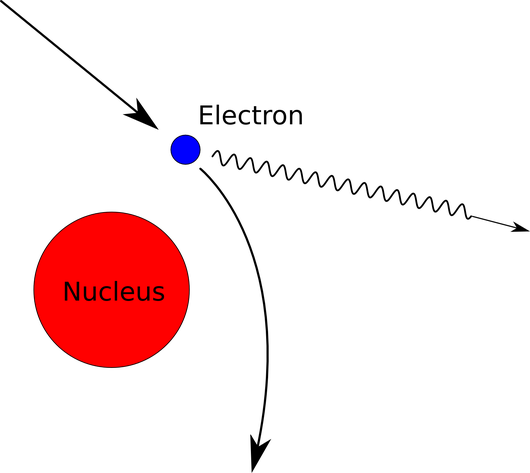
\includegraphics[width=0.3\textwidth]{images/bremsstrahlung.png}
%\caption{\label{plot.freefree} Schematic showing the physical process leading to free-free emission. As we can see, the electron is scattered, but not captured. Source: \url{https://thephysicsbehind.com/2015/04/16/x-ray-tubes/}}
%\end{figure*}

\pg
This emission's spectrum is heavily dependent on a number of factors: including frequency, temperature, and critically, free-free opacity $\tau_\nu$, itself a function of electron density. It is characterised by a knee in its spectrum, occurring where $\tau_\nu\sim 1$. This knee delineates two regions with different spectral indices; $\alpha \sim -0.1$ at higher frequencies, and $\alpha \leq 2$ at lower frequencies. This gives a characteristic shape, shown in Fig. \ref{plot.freefree.spectrum}.
\begin{figure*}[!h]
\centering
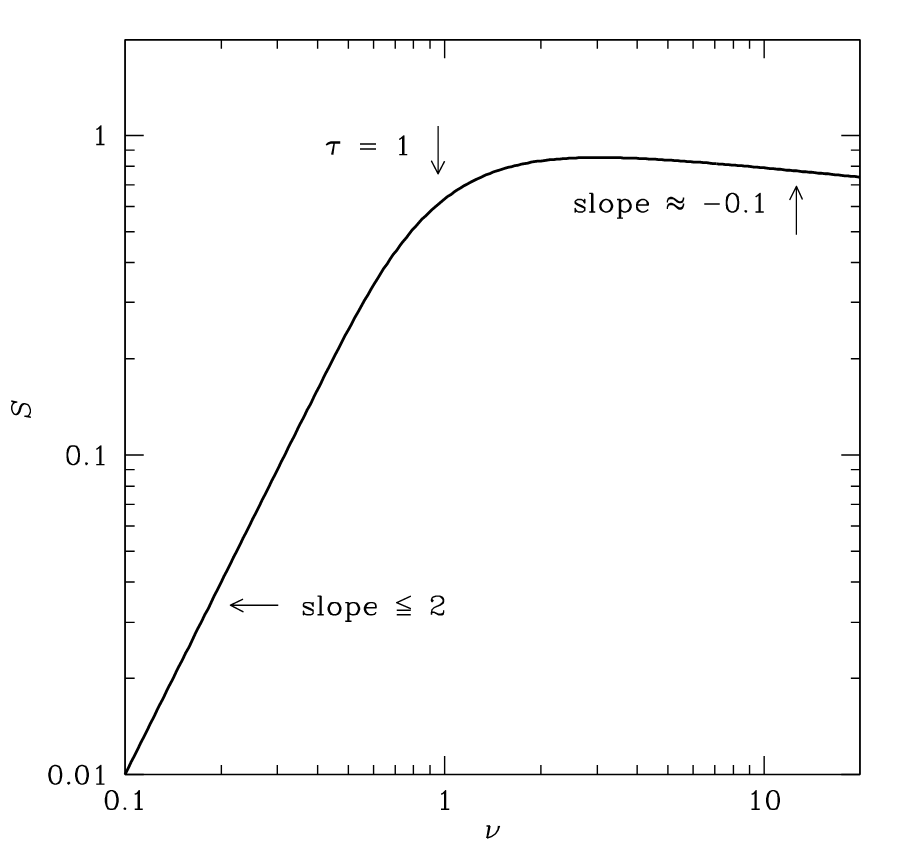
\includegraphics[width=0.9\textwidth]{images/freefree.png}
\caption{\label{plot.freefree.spectrum} Characteristic spectrum of free-free radiation. Arbitrary unit scale. Source: NRAO online course.}
\end{figure*}

\pg
As we can see, this spectrum falls off sharply with frequency. As such, while it is expected to dominate over thermal emission in the absence of synchrotron radiation, it is unlikely to dominate in the LOFAR band. It acts as a tracer for star formation and other "gentler" physical processes detected at low radio frequencies.

\subsection{Synchrotron Radiation}
\pg
Synchrotron radiation (or "magnetobremsstrahlung") occurs when the trajectory of a high-energy charged particle is deflected by a magnetic field. As the German name suggests, it is the magnetic equivalent of free-free radiation. It is the tracer of extremely violent processes, such as AGN jets. In its mildly relativistic regime, it is referred to as cyclotron radiation, after the device in which it was first tested, and in non-relativistic regimes, it is known as gyro radiation. 

\pg






\clearpage
\section{LOFAR: The LOw-Frequency Array}

\pg
In this section, we will describe the LOw Frequency Array LOFAR \citepads{2013A&A...556A...2V}, its technical properties and its current state of the art. In particular, the distinction between "Dutch" LOFAR and "international" LOFAR - and the technical problems associated with each - will be made explicit in this section.

\pg
LOFAR is a SKA pathfinder instrument, which means that it serves not only as a cutting-edge instrument in its own right, but does so with the explicit aim of serving as testing grounds for technologies \& techniques which could be usefully implemented in the SKA. It is in this context, for example, that trailblazers such as NeNuFar \citepads{2012sf2a.conf..687Z}, a low-frequency extension of LOFAR, are tested. LOFAR is an interferometric array, meaning that it consists of antennas which are combined to form stations, which are themselves distributed throughout the Netherlands and Europe.
\begin{figure}[h!] 
  \begin{minipage}[c]{0.45\linewidth}
    \centering
    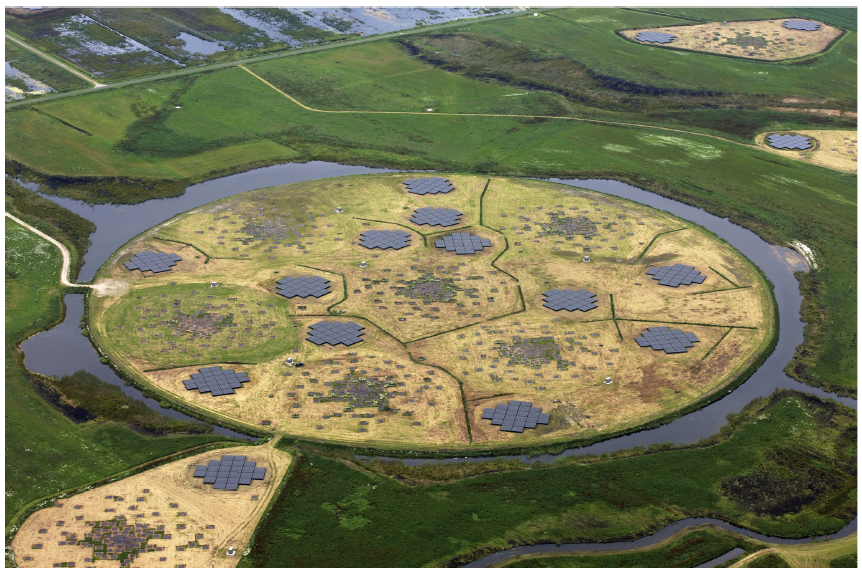
\includegraphics[width=\linewidth]{images/superterp.png}
	\subcaption{\label{fig.lofar.superterp} LOFAR core, known as the Superterp.}
%    \vspace{4ex}
  \end{minipage}
  \hfill
  \begin{minipage}[c]{0.45\linewidth}
    \centering
    \includegraphics[width=.5\linewidth]{images/{lofar-core-map_grey.jpg}}
    \subcaption{\label{fig.lofar.core} Distribution of the so-called LOFAR "core" stations, which include the Superterp.}
%    \vspace{4ex}
  \end{minipage} 
  \begin{minipage}[c]{0.45\linewidth}
    \centering
    \includegraphics[width=\linewidth]{images/{Distribution_Remote_Stations}} 
    \subcaption{\label{fig.lofar.remote} LOFAR with both "core" and "remote" stations.}
%    \vspace{4ex}
  \end{minipage}
  \begin{minipage}[c]{0.45\linewidth}
    \centering
    \includegraphics[width=.9\linewidth]{images/{Distribution_International_Stations}} 
    \subcaption{\label{fig.lofar.international} International LOFAR. Newer stations (one in Ireland, three in Poland) are not shown here.}
%    \vspace{4ex}
  \end{minipage} 
\caption{\label{fig.lofar.distribution} Geographic location and distribution of LOFAR stations, explicitly showing what is meant by Superterp, core, remote and international stations. All images from \href{https://www.astron.nl/radio-observatory/astronomers/users/technical-information/lofar-array-configuration/lofar-array-conf}{the official ASTRON website}}
\end{figure}


\pg
There are two bands to LOFAR, which are known as LOFAR-HBA (High-Band Antennas) and LOFAR LBA (Low-Band Antennas). \cref{fig.lofar.superterp,fig.fr606.layout} show the layout of the 6 innermost core stations and the French international LOFAR station, respectively.
\begin{figure}[h!]
\includegraphics[width=0.5\textwidth]{images/{LOFAR_NenuFAR.jpg}}
\caption{\label{fig.fr606.layout} Layout of FR606, the French LOFAR station at Nancay. At bottom left are the HBA tiles, bottom right the LBA dipoles, and at the top are some of the NenuFAR mini-arrays.}
\end{figure}



\pg
We see the presence, in both cases, of two very different antenna types. One of these antenna types is not a single antenna, but rather a phased array: 16 antenna dipoles distributed in a $4 \times 4$ array. LOFAR stations include 48 such tiles, distributed in a cross pattern. This pattern is shown in \cref{fig.hba.tile}. Core stations HBA tiles are split into two 24-tile crosses. The antennas from each tile are combined into a phased array with a single ``tile beam", and all tile beams are themselves combined into a station beam\footnote{Referece: \href{https://www.astron.nl/radio-observatory/astronomers/technical-information/antennae/antennae-description}{ASTRON technical description}}. This station beam is then pointed digitally.
\begin{figure}[h!]
\includegraphics[width=0.45\textwidth]{images/{Schematic-diagram-of-a-24-tile-LOFAR-HBA-station-A-tile-is-made-of-16-dual-polarization.png}}
\caption{\label{fig.hba.tile} Layout of a single HBA tile. Source: \href{https://www.researchgate.net/profile/Sarod_Yatawatta/publication/281316394/figure/fig1/AS:614002589720576@1523401033149/Schematic-diagram-of-a-24-tile-LOFAR-HBA-station-A-tile-is-made-of-16-dual-polarization.png}{Sarod Yatawatta researchgate profile}}
\end{figure}

\pg
LOFAR-HBA is sensitive to higher frequencies, from 120 MHz to 240 MHz\footnote{Reference: \href{http://www.lofar.org/about-lofar/system/lofar-numbers/lofar-numbers}{LOFAR.org website}}. It has a smaller field of view than LOFAR-LBA, but a better resolution. 

\pg
LBA antennas, meanwhile, follow a very simple - and cost-effective - design. A typical LBA antenna is shown in \cref{fig.lba.ant}. 96 such antennas are spread in a semi-random pattern in each LOFAR station\footnote{Reference: \href{http://www.lofar.org/about-lofar/system/lofar-numbers/lofar-numbers}{LOFAR.org website.}}. In survey observations, they are combined as a single phased array.
\begin{figure}[h!]
\includegraphics[width=0.45\textwidth]{images/{lba.png}}
\caption{\label{fig.lba.ant} Picture of a single LBA antenna. Source: \href{https://i2.wp.com/lofar.ie/wp-content/uploads/2017/04/lba.png?resize=1500\%2C1000}{LOFAR technology website.}}
\end{figure}

\pg
The dipole design frees observers from the need to physically point antennas at all: the final station pointing is achieved by digitally introducing delays in observed phase before averaging the data. In this sense, the pointing is achieved in the same way as individual HBA tile pointing, but with one less degree of complexity. These antennas are receptive to signals emitted in the 30-80 MHz frequency range.

\pg
At the time of writing, use of the LBA data is still relatively new, as its calibration is a very tricky problem. For similar reasons, international LOFAR (i.e. the full LOFAR array) has not been used, at the time of writing, to create wide-field survey images. A large part of the work described in this manuscript consists of reaching a point where full use can be made of international LOFAR, in a streamlined and repeatable way. 

